67. $\cfrac{(x^2+4x-1)(x^2+8x+16)}{(x^2-x)(x^2+16x+64)}\geqslant0\Leftrightarrow
\cfrac{(x-(-2-\sqrt{5}))(x-(\sqrt{5}-2))(x+4)^2}{x(x-1)(x+8)^2}\geqslant0.$ Применив метод интервалов, найдём ответ: $x\in
(-\infty;-8)\cup(-8;-2-\sqrt{5}]\cup\{-4\}\cup(0;\sqrt{5}-2]\cup(1;+\infty).$
\begin{figure}[ht!]
\center{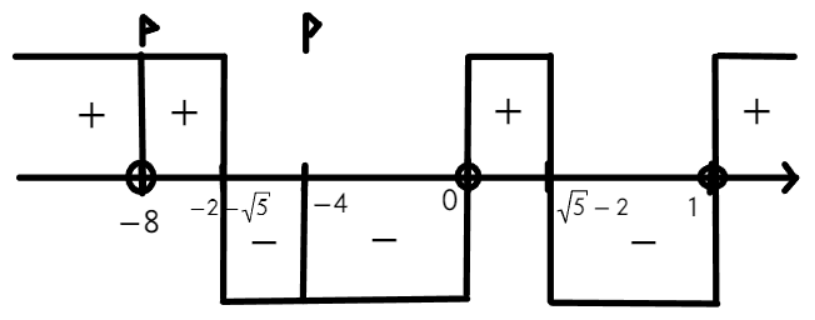
\includegraphics[scale=0.35]{ner9-67.png}}
\end{figure}\\
